\documentclass{beamer}
\usepackage[russian]{babel}
\usetheme{metropolis}

\usepackage{amsthm}
\setbeamertemplate{theorems}[numbered]

\setbeamercolor{block title}{use=structure,fg=white,bg=gray!75!black}
\setbeamercolor{block body}{use=structure,fg=black,bg=gray!20!white}

\usepackage[T2A]{fontenc}
\usepackage[utf8]{inputenc}

\usepackage{hyphenat}
\usepackage{amsmath}
\usepackage{graphicx}

\setbeamercovered{transparent}

\AtBeginEnvironment{proof}{\renewcommand{\qedsymbol}{}}{}{}

\title{
Микроэкономика-I
}
\author{
Павел Андреянов, PhD
}

\begin{document}

\maketitle

\section{Квиз}

\begin{frame}{Квиз}

\begin{itemize}
  \item Чем знаменит Жерар Дебрё? \pause
  \item Докажите что минимум вогнутых функций вогнутый. \pause
  \item Приведите пример квазивогнутой но не вогнутой функции. \pause
  \item Когда Пете было 19 лет, он пошел учиться в универе, хотя мог пойти работать. Однако, через 4 года (бакалавр), он стал работать и продолжать учиться одновременно. Является ли это нарушением WARP? Поясните.  \pause
  \item Что такое выпуклая задача? \pause
  \item Назовите три аксиомы рациональности. \pause
  \item Какие из нижеперечисленных функций являются монотонны и/или (квази-)вогнутыми в $\mathbb{R}^1_+$: $$x, \ x^2, \ x^3, \ \sin(x), \ \log(x), \ \sqrt{x}, \ x^2 + x, \ \sqrt{x} + x?$$
\end{itemize}

\end{frame}

\section{План}

\begin{frame}{План}

Первая половина лекции посвящена классической постановке задачи потребителя с так называемым (линейным) бюджетным множеством.

Мы поговорим подробно о Методе Множителей Лагранжа. Формулировки теорем знать необязательно, но хотелось бы, чтобы вы примерно представляли, что происходит.

Потом перерыв.

Во второй половине лекции будут введены термины спроса и косвенной полезности и некоторые сопутствующие определения и свойства.

\end{frame}


\section{Бюджетное ограничение}

\begin{frame}{Бюджетное ограничение}

Наиболее часто в нашем курсе будет встречаться классическое (линейное) \alert{бюджетное ограничение}:
$$ B(x,y) = p x + q y - I \leqslant 0$$
где $p, q \geqslant 0$ - это цены товаров, а $I \geqslant 0$ - это бюджет. 

Для экспозиции я все показываю в пространстве (портфелей) товаров $\mathbb{R}^2_+$, но ничего не мешает вам обобщить это в $\mathbb{R}^n_+$. 

Еще я буду иногда обозначать само \alert{бюджетное множество} как $$B(p,q,I)=\{x,y \in \mathbb{R}^2_{+}| \ px + qy \leqslant I\},$$ смотрите на контекст.

\end{frame}

\begin{frame}{Бюджетное ограничение (2d)}

\begin{figure}[hbt]
\centering
\includegraphics[width=.8 \textwidth]{budget_2d.png}
\end{figure}

\end{frame}

\begin{frame}{Бюджетное ограничение (3d)}

\begin{figure}[hbt]
\centering
\includegraphics[width=.8 \textwidth]{budget_3d.png}
\end{figure}

\end{frame}

\begin{frame}{Бюджетное ограничение}

Откуда берутся координаты концов треугольника?

\begin{itemize}
  \item Пересечение $p x + q y - I$ с $x=0$ дает $y = I/q$
  \item Пересечение $p x + q y - I$ с $y=0$ дает $x = I/p$
\end{itemize}

Попробуйте представить себе как деформируется бюджетное множество при изменении параметров $p,q,I$.

\end{frame}

\begin{frame}{Бюджетное ограничение}

Обычно, значения цен и бюджетов: $p,q,I \geqslant 0$. 

Вопрос: при каких значениях $p,q,I$ бюджетное множество компактно? Непусто? 

Что это значит в контексте Теоремы Вейерштрасса?

\end{frame}

\begin{frame}{Бюджетное ограничение}

Покажем, что бюджетное множество <<монотонно>> по $p,q,I$.

\begin{itemize}
  \item Если $p'<p$ то $B(p,q,I) \subset B(p',q,I)$,
  \item Если $I<I'$ то $B(p,q,I) \subset B(p,q,I')$.
\end{itemize}

Изменение цены выглядит как <<вращение>> бюджетного множества вокруг точки, а изменение бюджета как <<отодвигание>> бюджетной линии.

Отсюда, в частности, следует что полезность в оптимуме не может упасть при увеличении бюджета или уменьшении любой из цен, ведь потребитель может всегда может достигнуть, как минимум, старого уровня полезности.

\end{frame}

\begin{frame}{Бюджетное ограничение}

В этом курсе мы будем зачастую нормализовать параметры $p,q,I$ одним из следующих способов:

\begin{itemize}
  \item прибить последнюю цену к единице: $q = 1$
  \item прибить бюджет к единице: $I = 1$
  \item прибить цены к симплексу: $p + q = 1$
\end{itemize}

Интерпретация этого - переход к безразмерным величинам:
$$ p,q,I \to \frac{p}{p+q},\frac{q}{p+q},\frac{I}{p+q}$$
за счет деления всех денежных параметров на константу.

\end{frame}

\section{Метод Лагранжа}

\begin{frame}{Метод Лагранжа}

\begin{columns}
\begin{column}{0.5\textwidth}
   \alert{Джозеф-Луи Лагранж} (Giuseppe Luigi Lagrangia) итальяно-французский математик второй половины 18 века. Работал над основами теоретической механики, в процессе разработав вариационный анализ, а также популяризовав (уже известный до него) так называемый \alert{метод множителей Лагранжа}.
\end{column}
\begin{column}{0.5\textwidth}  %%<--- here
    \begin{center}
     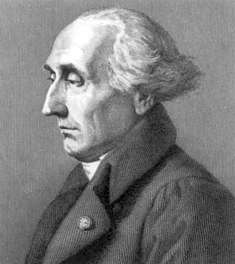
\includegraphics[width=1\textwidth]{Lagrange.png}
     \end{center}
\end{column}
\end{columns}

\end{frame}

\begin{frame}{Метод Лагранжа}

Запишем нашу оптимизационную задачу в следующем виде:
$$ U(x, y) \to \max_{(x,y) \in \mathbb{R}^2_{+}} \quad s.t.\quad  B(x,y) \leqslant 0$$
Тогда \alert{Лагранжиан} принимает вид:
$$ \mathcal{L}(x, y | \lambda) = U(x,y) - \lambda B(x,y)$$
Знак перед множителем Лагранжа важен в доказательствах, но на практике не играет роли и можно ставить любой.

Традиция такова, что $\lambda I$ должен войти с плюсом, так чтобы частная производная по бюджету была равна множителю $\lambda$.

\end{frame}

\begin{frame}{Метод Множителей Лагранжа}

Далее алгоритм предписывает найти седловую точку Лагранжиана в пространстве $(x, y, \lambda)$:
$$ \mathcal{L}'_x = 0, \quad \mathcal{L}'_y = 0, \quad \mathcal{L}'_{\lambda} = 0.$$
Это система из трех уравнений с тремя неизвестными.

Таким образом, задача условной оптимизации сводится к безусловной. Однако не совсем понятно, почему метод Лагранжа вообще работает.

\end{frame}

\section{Выпуклая интерпретация ММЛ}

\begin{frame}{Выпуклая интерпретация ММЛ}

Если Лагранжиан (квази-)вогнутый по товарам $x,y$ то можно применить  так называемую \alert{сильную дуальность} или \alert{сильный принцип Лагранжа}.

Сам Лагранж к этому отношения не имеет, эти идеи были разработаны гораздо позже, в 20 веке.
\end{frame}

\begin{frame}{Фон Нейман}

\begin{columns}
\begin{column}{0.5\textwidth}
   \alert{Джон фон Нейман} (John von Neumann) венгро-американский математик первой половины 20 века. Работал над многочисленными областями математики и физики, в том числе \alert{интерпретацией Лагранжевой дуальности при помощи теории игр} и ядерной программой США.
\end{column}
\begin{column}{0.5\textwidth}  %%<--- here
    \begin{center}
     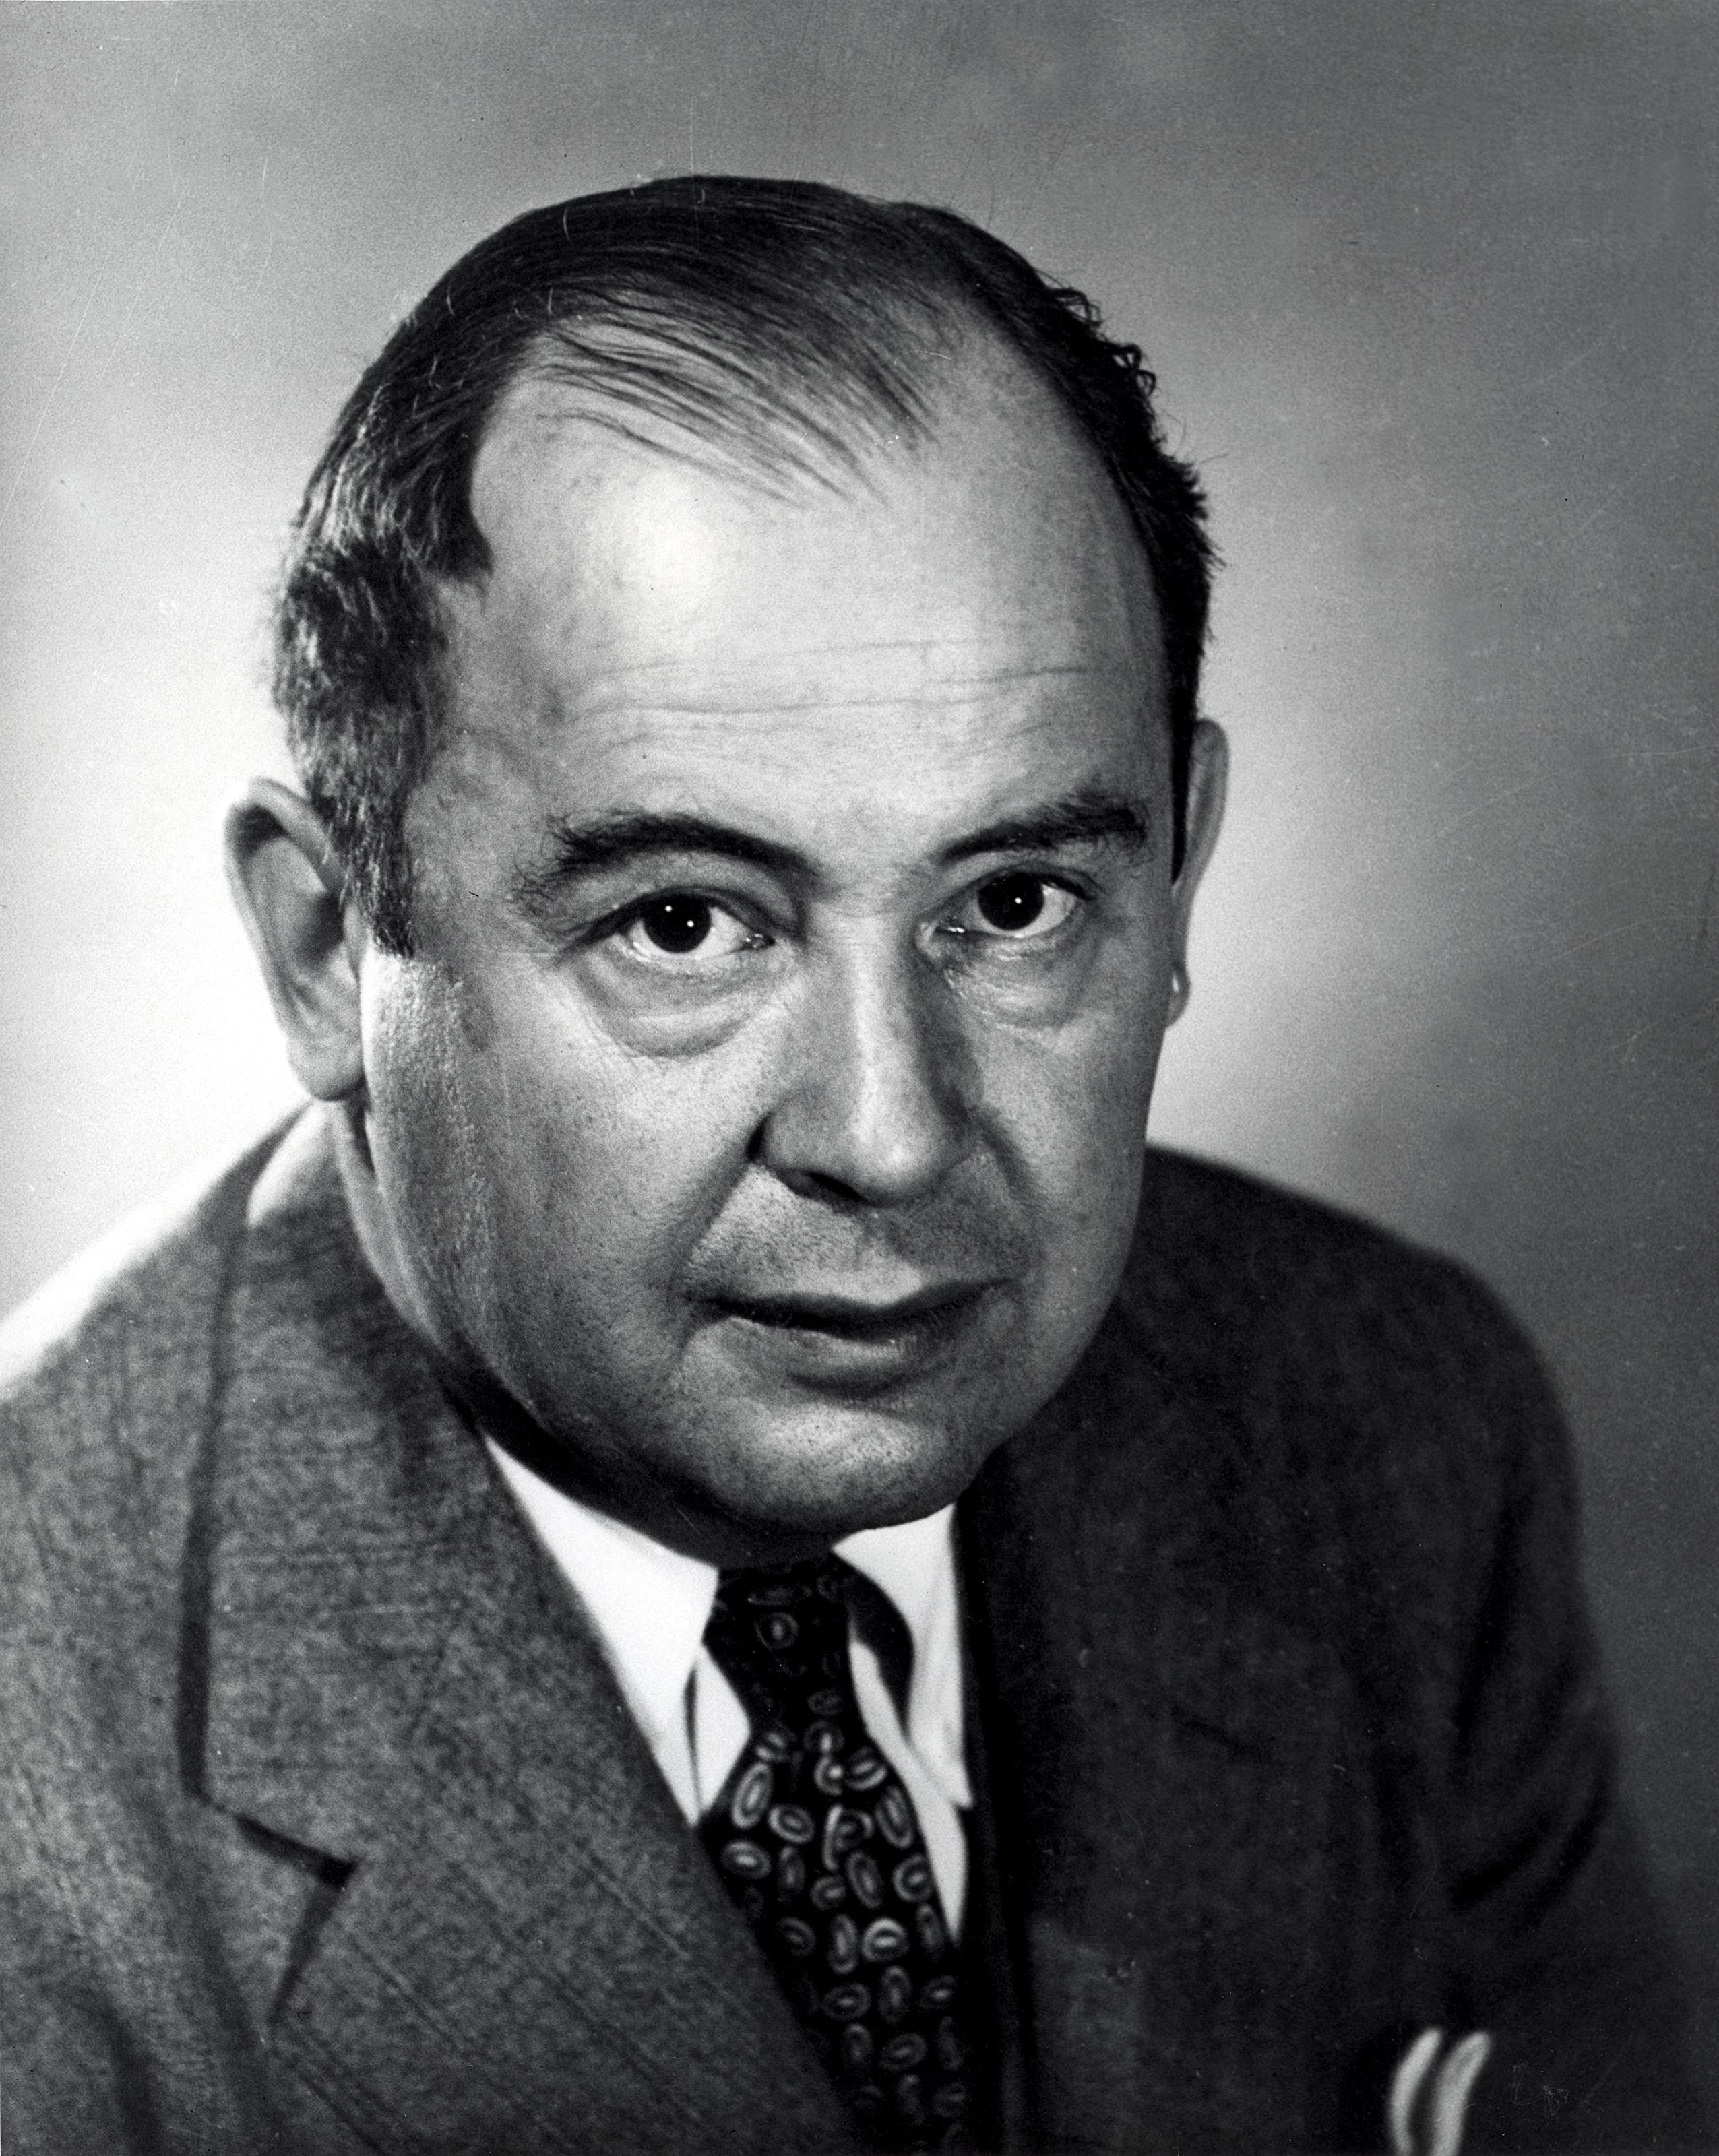
\includegraphics[width=1\textwidth]{neuman.jpg}
     \end{center}
\end{column}
\end{columns}

\end{frame}

\begin{frame}{Выпуклая интерпретация ММЛ}

$$ \min_{\lambda \geqslant 0} \max_{x(\lambda),y(\lambda) \geqslant 0} \mathcal{L}(x,y | \lambda) = \textcolor{red}{\max_{x,y \geqslant 0} \min_{\lambda(x,y) \geqslant 0} \mathcal{L}(x,y | \lambda)} $$ 

Справа стоит негладкая задача, эквивалентная условной оптимизации. Этот совершенно не очевидный факт можно понять как равновесие в игре с двумя агентами.

Первым ходит потребитель, он выбирает $(x,y)$. Лагранж отвечает ему множителем так чтобы сделать похуже, а именно, $\lambda(x,y) = \infty$ если $B(x,y) > 0$, и $\lambda(x,y) = 0$ если $B(x,y) \leqslant 0$. 

Потребитель удерживается в ограничении, при этом максимизируя оригинальную полезность $\mathcal{L}(x,y | 0) = U(x,y)$.

\end{frame}

\begin{frame}{Выпуклая интерпретация ММЛ}

$$ \textcolor{red}{\min_{\lambda \geqslant 0} \max_{x(\lambda),y(\lambda) \geqslant 0} \mathcal{L}(x,y | \lambda)} =  \max_{x,y \geqslant 0} \min_{\lambda(x,y) \geqslant 0} \mathcal{L}(x,y | \lambda) $$ 

Слева стоит гладкая задача, у которой есть одна критическая точка типа <<седло>>, а значит его можно найти обыкновенными условиями первого порядка:
$$ \nabla_{(x,y)} \mathcal{L} = 0, \quad \nabla_{\lambda} \mathcal{L} = 0.$$

В выпуклом случае (квазивогнутая полезность + выпуклое ограничение) координаты решения двух задач, а также значение целевой функции совпадают, это называется \alert{теоремой о Минимаксе}, или сильной (Лагранжевой) дуальностью.

\end{frame}

\section{Невыпуклая интерпретация ММЛ}

\begin{frame}{Условия Каруш-Кун-Такера и Фриц-Джона}

\begin{columns}
\begin{column}{0.5\textwidth}
   \alert{Вильям Каруш, Харольд Кун и Альберт Такер} это три разных американских математика, которым приписывают разработку необходимых и достаточных условий в задачах оптимизации с ограничениями. Историки математики также отметят незаслуженно забытого \alert{Фриц Джона} (!!!это один человек!!), работа которого очень близка по духу к ККТ.
\end{column}
\begin{column}{0.5\textwidth}  %%<--- here
    \begin{center}
     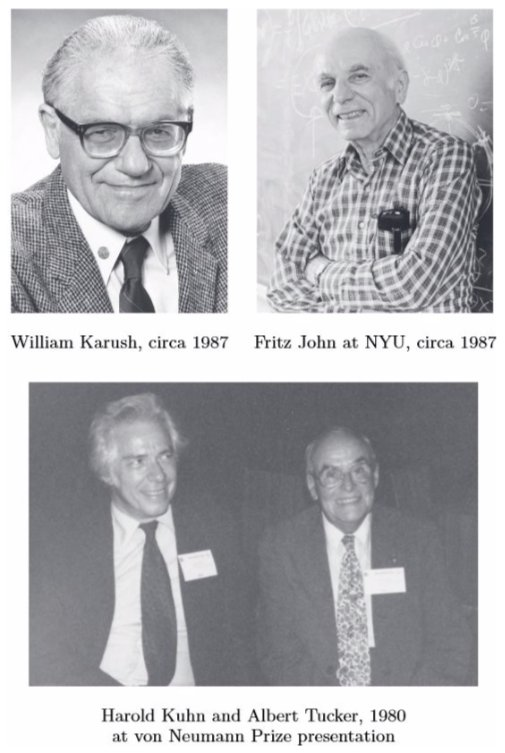
\includegraphics[width=1\textwidth]{kktf}
     \end{center}
\end{column}
\end{columns}

\end{frame}

\begin{frame}{Невыпуклая интерпретация ММЛ}


Основная идея такова, что градиент целевой функции и градиент активного ограничения должны быть параллельны друг другу:
$$ \nabla_{(x,y)}U - \lambda \nabla_{(x,y)} B = 0$$

Это называется необходимыми условиями первого порядка, или сокращенно \textbf{УПП} (в англ. \textbf{FOC}). 

Удивительным образом это совпадает с поиском седловой точки Лагранжиана.

\end{frame}

\begin{frame}{Невыпуклая интерпретация ММЛ}

Далее надо сделать еще один шаг и проверить достаточные условия второго порядка, или сокращенно \textbf{УВП} (в англ. \textbf{SOC}):
$$ \nabla^2_{(x,y)}U - \lambda \nabla^2_{(x,y)} B \leqslant 0$$
на касательном к ограничении пространстве. 

Еще более удивительным образом это совпадает с проверкой квазивогнутости Лагранжиана в точке. Убедиться можно, например, через окаймленный Гессиан.

Наконец, всякие Qualification Constraints тривиально выполнены для линейных бюджетных множеств.

\end{frame}

\section{Геометрическая интерпретация ММЛ}

\begin{frame}{Геометрическая интерпретация ММЛ}

Если мы каким то образом убедили себя что решение находится <<внутри бюджетной линии>>, например, за счет комбинации фактов

\begin{itemize}
  \item $U$ локально ненасыщаема в $\mathbb{R}^n_+$
  \item $U = -\infty$ на границе $\mathbb{R}^n_+$
\end{itemize}

То оптимум находится просто \alert{в точке касания} бюджетной линии и линии уровня полезности, что характеризуется сонаправленностью их градиентов:
$$ \nabla_{(x,y)} U = \lambda \cdot \nabla_{(x,y)} B.$$

Ясно, что это те же самые условия, что поиск седла у Фон Неймана или условия Каруш-Куна-Такера.

\end{frame}

\begin{frame}{Геометрическая интерпретация ММЛ}

\begin{figure}[hbt]
\centering
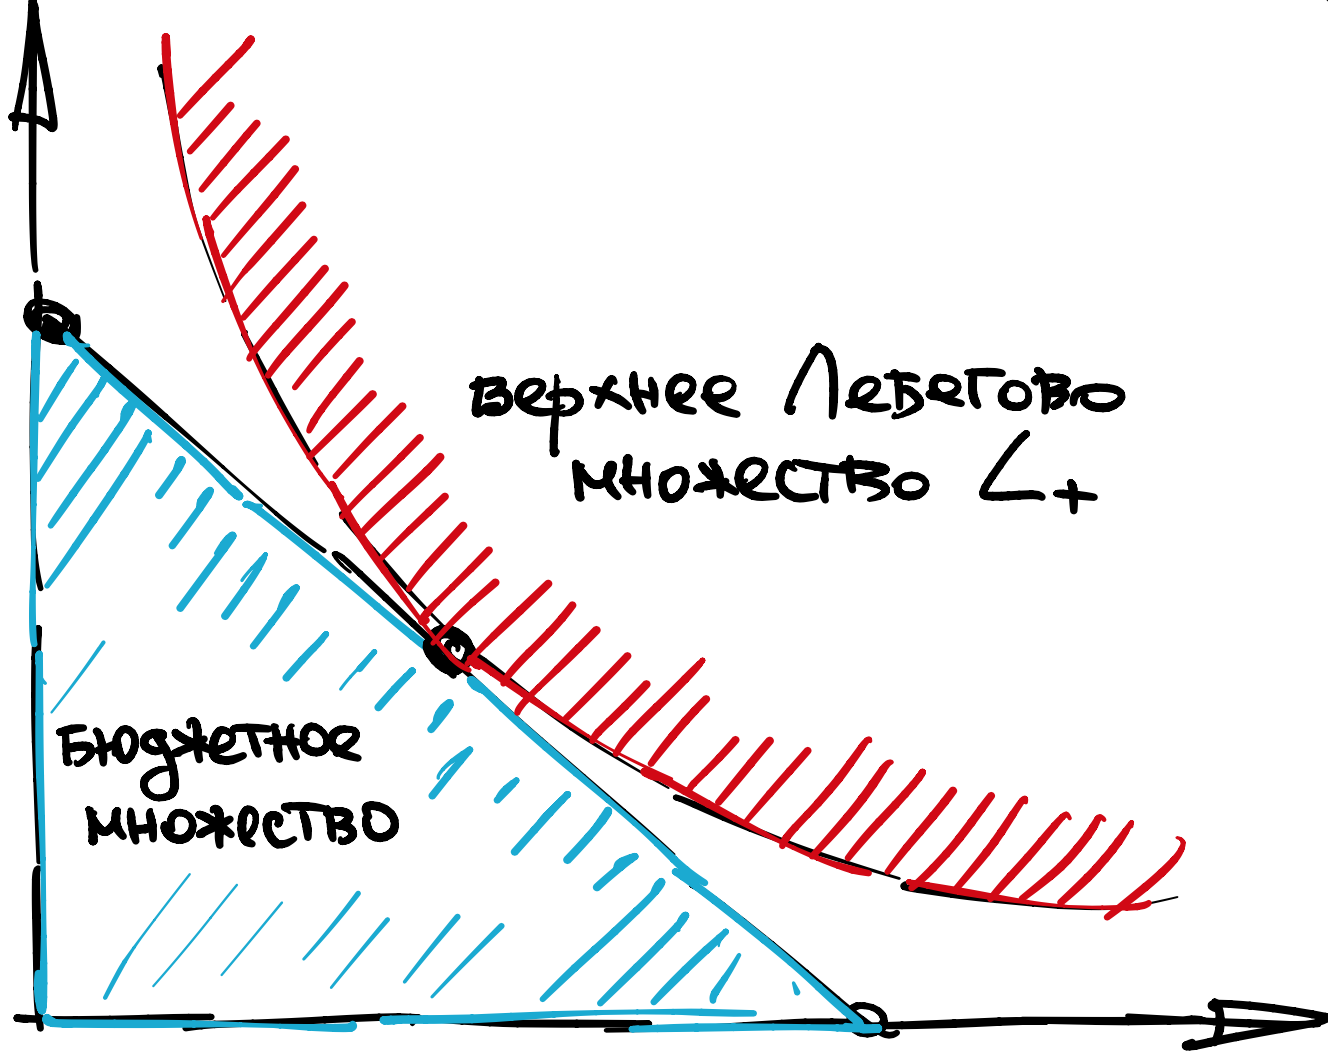
\includegraphics[width=.8 \textwidth]{tangency.png}
\end{figure}

\end{frame}

\section{Угловые решения}

\begin{frame}{Угловые решения}

На самом деле, поскольку мы оптимизируем в $\mathbb{R}^n_{+}$ в Лагранжиан, стоило бы добавить еще дополнительные члены, по одному на каждый товар. 
$$ \mathcal{L}(x,y | \lambda, \gamma, \delta) = U(x,y) - \lambda B(x,y) - \gamma x - \delta y$$
Однако, в экономических приложениях, как правило, решение внутреннее, поэтому мы этого делать никогда не будем.

С другой стороны, \alert{если решение ожидается на границе} (как с линейной полезностью) \alert{его можно отыскать непосредственно перебором по остриям бюджетного множества}.

\end{frame}

\section{Значение Лагранжиана в оптимуме}

\begin{frame}{Значение Лагранжиана в оптимуме}

Вспомним условие невязки из курса мат. анализа:
$$ \lambda^{\ast} B(x^{\ast},y^{\ast}) = 0.$$
Оно означает, что одно из двух обязательно верно: 

\begin{itemize}
  \item либо $\lambda^{\ast}$ равен нулю, тогда полезность максимизируется внутри бюджетного множества, как если бы ограничения не было.
  \item либо $\lambda^{\ast}$ положительный, тогда полезность максимизируется (как бы) снаружи,  но тогда и ограничение выполнено с равенством.
\end{itemize}
 

\end{frame}

\begin{frame}{Значение Лагранжиана в оптимуме}

В любом случае, получается что в оптимуме значение Лагранжиана совпадает со значением целевой функцией:
$$ \mathcal{L}(x^{\ast}, y^{\ast} | \lambda^{\ast}) = U(x^{\ast}, y^{\ast}) - \lambda^{\ast} B(x^{\ast}, y^{\ast})$$ 
Это очень полезное свойство, запомним его.

\end{frame}

\section{Интерпретация $\lambda$}

\begin{frame}{Интерпретация $\lambda$}

У множителя $\lambda$ в Лагранжиане есть особая экономическая интерпретация - это \alert{теневая цена} нарушения ограничения:
$$\mathcal{L} = U(x,y) - \lambda \cdot B(x,y), \quad B(x,y) \leqslant 0$$ 
Если вам очень хочется выйти за ограничение, открывается черный рынок на котором продается возможность это сделать по цене $\lambda \cdot B(x,y)$. Далее цена на рынке должна выстроиться таким образом, чтобы вы покупали ровно 0 единиц этого <<товара>>, как говорит условие невязки. 

Это и будет правильный множитель Лагранжа.
\end{frame}

\section{Перерыв 15 минут}

\section{Кривые спроса}

\begin{frame}{Кривые спроса}

Нас будут интересовать координаты оптимума $x^{\ast}(p,q,I)$, $y^{\ast}(p,q,I)$ в задаче максимизации полезности при бюджетном ограничении, как функции (кривые) от цен $p,q$ и бюджета $I$. 

Они также называются \alert{функциями (кривыми) спроса}.

\begin{definition}
Функции спроса делятся на кривые \alert{цена-потребление} $x^{\ast}(p)$, $y^{\ast}(q)$ и кривые \alert{доход-потребление} $x^{\ast}(I)$, $y^{\ast}(I)$.
\end{definition}

Есть еще 2 другие группы кривых: общие расходы $p x^{\ast}(I)$, $q y^{\ast}(I)$, и доли расходов $p x^{\ast}(I)/I$, $q y^{\ast}(I)/I$, как функции от дохода, называются \alert{кривыми Энгеля}.

\end{frame}

\begin{frame}{Кривые Энгеля}

\begin{columns}
\begin{column}{0.5\textwidth}
   \alert{Эрнст Энгель} (Ernst Engel) немецкий математик и статистик 19 века, автор \alert{закона (парадокса) Энгеля}, утверждающего, что расходы на продукты питания растут с доходом, а доля этих расходов в общем бюджете, наоборот, падает. 
\end{column}
\begin{column}{0.5\textwidth}  %%<--- here
    \begin{center}
     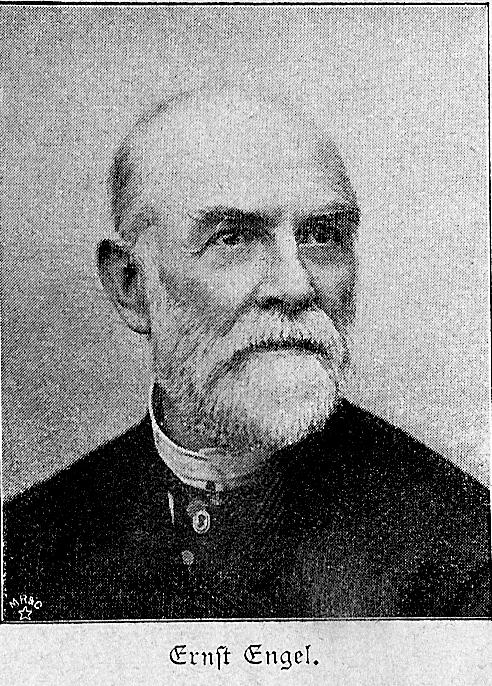
\includegraphics[width=1\textwidth]{engel.jpeg}
     \end{center}
\end{column}
\end{columns}

\end{frame}

\begin{frame}{Кривые Энгеля}

\begin{figure}[hbt]
\centering
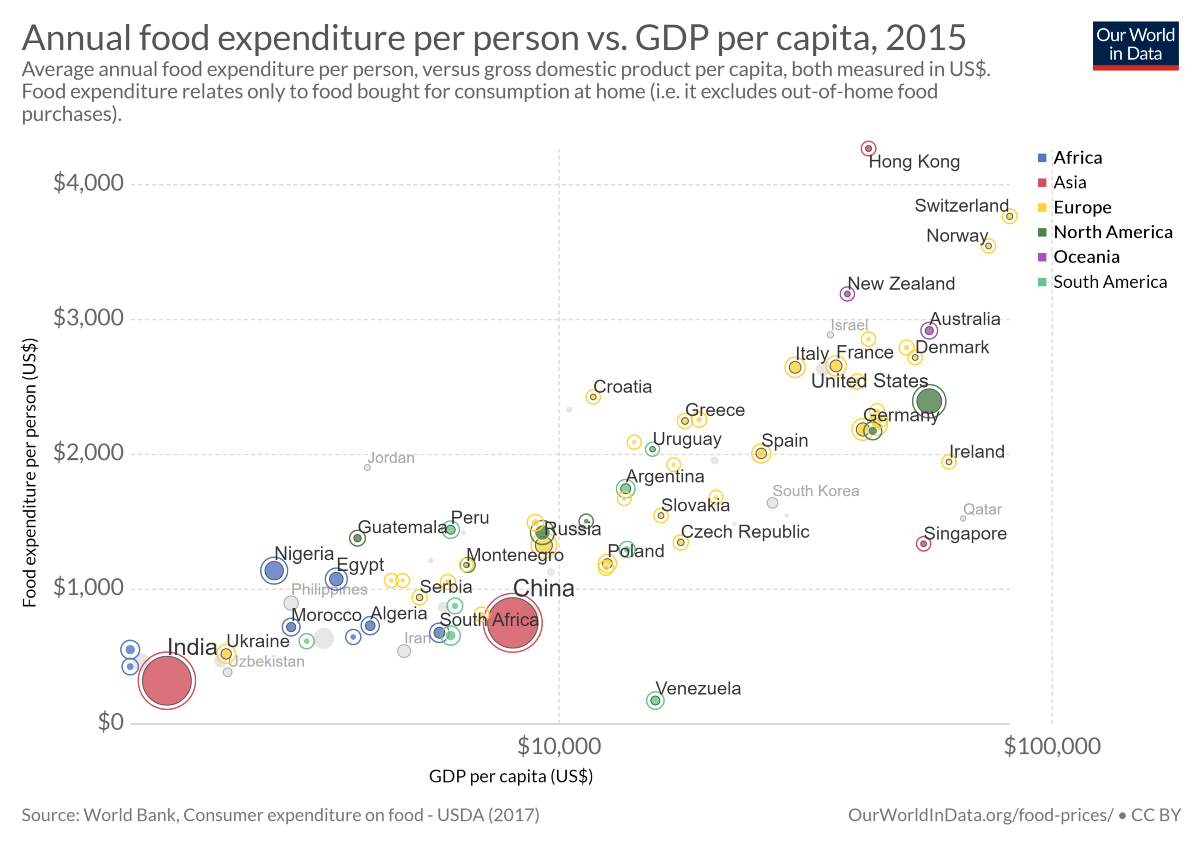
\includegraphics[width=1 \textwidth]{worldbank.png}
\end{figure}

\end{frame}

\begin{frame}{Кривые Энгеля}

\begin{figure}[hbt]
\centering
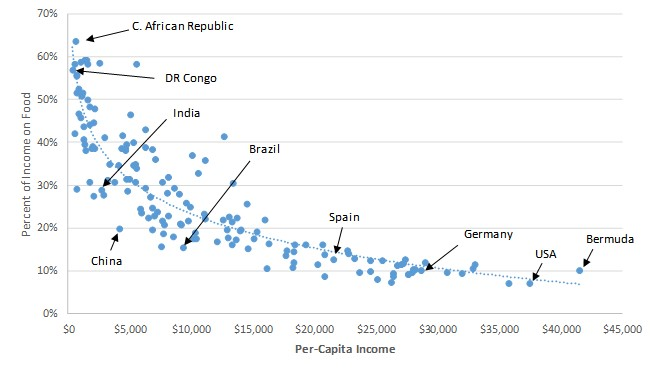
\includegraphics[width=1 \textwidth]{worldbank2.jpeg}
\end{figure}

\end{frame}

\begin{frame}{Кривые Энгеля}

Более того, люди более охотно отвечают на вопрос о доле, чем об их доходе, поэтому это просто классная мера бедности населения с точки зрения проведения соц. опроса.

Доля расходов на продукты питания в бюджете называется \alert{коэффициентом Энгеля} и используется для категоризации уровня жизни стран:

\begin{itemize}
  \item $>50\%$ низкий уровень жизни  
  \item 40-50\% средний уровень жизни
  \item 30-40\% хороший уровень жизни
  \item $<30\%$ высокий уровень жизни
\end{itemize}

Пока богатые развитые страны таргетируют инфляцию, бедные и развивающиеся страны таргетирут коэффициент Энгеля.

\end{frame}


\section{Нормальные и инфериорные товары}

\begin{frame}{Нормальные товары}

Сфокусируемся на наклонах кривых доход-потребление.

\begin{definition}
\alert{Нормальными товарами} называются товары, кривые спроса которых монотонно возрастают по доходу, то есть:
$$\frac{\partial x^{\ast}}{\partial I} \geqslant 0.$$
\end{definition}
Проверка нормальности при аккуратно выведенных кривых спроса - это механическое упражнение в дифференцировании. 

Как правило, подразумевается глобальное свойство, но можно, в принципе, говорить о локальной нормальности, то есть, в окрестности какой то точки $(p,q,I)$.

\end{frame}

\begin{frame}{Инфериорные товары}

Считается, что большая часть товаров - нормальны, однако, есть исключения.

\begin{definition}
Товар, у которого нормальность нарушается:
$$\frac{\partial x^{\ast}}{\partial I} < 0,$$ 
называется \alert{инфериорным} (при этих значениях параметров). 
\end{definition}

Инфериорность всегда подразумевается локально, так как \alert{глобально инфериорных товаров не бывает}. Действительно, при уменьшении бюджета вы просто не можете постоянно увеличивать спрос, вы вылетите за границу бюджета.

\end{frame}

\begin{frame}{Инфериорные товары}

Интуитивно, инфериорность (от англ. \textit{inferior}) означает что ваш товар $x$ является худшим по отношению к какому-то другому товару $y$. Например, хлеб и консервы считаются инфериорными по отношению к красному мясу и рыбе. 

Когда бюджет растет, вы тратите большую часть дохода на дорогие мясо и рыбу, и меньшую на дешевые хлеб и консервы, а также потребляете их меньше в штуках. 

Любопытно, что чтобы сломать нормальность $x$, обязательно должен быть хотя бы один другой нормальный (в этой точке) товар $y$, по отношению к которому $x$ будет инфериорным (в этой точке).

\end{frame}

\begin{frame}{Доказательство}

\begin{lemma}
Все товары не могут быть одновременно инфериорными, хотя бы один точно нормальный.
\end{lemma}

Если бюджетное ограничение таково, что оптимум находится на бюджетной линии, то, дифференциируя $B(x,y)= 0$ по $I$, мы получаем: 
$$ p \frac{\partial x^{\ast}}{\partial I}  + q \frac{\partial y^{\ast}}{\partial I}  = 1.$$ 

Поскольку цены неотрицательные, то инфериорность всех товаров означала бы, что слева стоит отрицательное число, а справа единица, что есть противоречие.

\end{frame}

\begin{frame}{Инфериорные товары}

Определите какой из этих товаров инфериорный

\begin{itemize}
  \item бургер и картошка фри vs риб ай стейк
  \item поездки в такси vs личный автомобиль
  \item телефон-андройд vs айфон
  \item окко, айви vs netflix, hbo
\end{itemize}

Еще раз повторю, что сам по себе товар не может быть инфериорным, нужен обязательно какой-то другой товар, на который будет перекладываться траты. 

\end{frame}

\section{Субституты и комплементы}

\begin{frame}{Субституты}

Считается, что \alert{все товары в той или иной степени замещаемы}, некоторые больше некоторые меньше. 

Некоторые пары товаров особенно выделяются в этом плане, например: пепси и кола, лыжи и сноуборд, картошка фри и картошка по-деревенски... 

Если цена одного такого товара в паре сильно вырастет, то спрос на второй товар скорее всего вырастет, за счет покупателей, сбежавших от первого товара.

Такие товары называются субститутами.

\end{frame}

\begin{frame}{Субституты}

\begin{definition}
\textbf{\alert{Субститутами}} (gross substitutes) называются пары товаров, кривые спроса которых монотонно возрастают по ценам друг друга, то есть
\begin{itemize}
  \item $x$ субститут к $y$, если $\frac{\partial x^{\ast}}{\partial q} \geqslant 0,$
  \item $y$ субститут к $x$, если $\frac{\partial y^{\ast}}{\partial p} \geqslant 0.$
\end{itemize}
\end{definition}

Поразительно, но отношение субститутабильности на парах товаров может быть не симметричным.

\end{frame}

\begin{frame}{Заголовок в газетах}

\textit{...Необычайная засуха в Калифорнии привела к дефициту воды и подорожанию свежих апельсинов и мандаринов на 18\%... Производители соков (не только апельсиновых, но также яблочных и других) из импортных концентратов собрались на экстренное собрание для обсуждения мер предотвращения дефицита.}

Почему они так сделали?

\end{frame}

\begin{frame}{Комплементы}

У некоторых пар товаров наблюдается прямо противоположное свойство, их обычно покупают вместе, например: кайак и весло, компьютер и монитор...  

Если цена одного такого товара в паре сильно вырастет, то спрос на второй товар скорее всего упадет. 

Такие товары называются комплементами.

\end{frame}

\begin{frame}{Комплементы}

\begin{definition}
\alert{Комплементами} (gross complements) называются пары товаров, кривые спроса которых монотонно убывают по ценам друг друга, то есть 

\begin{itemize}
  \item $x$ комплемент к $y$, если $\frac{\partial x^{\ast}}{\partial q} < 0,$
  \item $y$ комплемент к $x$, если $\frac{\partial y^{\ast}}{\partial p} < 0.$
\end{itemize}
\end{definition}

Это отношение также не является симметричным.

\end{frame}

\begin{frame}{Заголовок в газетах}

\textit{Чтобы увеличить долю на рынке, цены на основную линейку смартфонов Самсунг были уменьшены 25\%. Компания-производитель чехлов для смартфонов неожиданно оказалась в списке <<единорогов>>.}

Что произошло?

\end{frame}

\begin{frame}{Мысли вслух}

К сожалению, субституты/комплементы не является симметричным свойством, то есть $x$ может быть субститутом к $y$, но $y$ при этом может оказаться комплементом к $x$. 

Это сигнализирует нам о том, что определение выбрано не совсем удачно. Мы к этому вернемся в лекции 4.

\end{frame}

\section{Товары Веблена и Гиффена}

\begin{frame}{Товары Веблена и Геффена}
Считается, что наклон кривой цена-потребление, как правило отрицательный. Другими словами, $$\frac{\partial x^*}{\partial p} <0, \quad \frac{\partial y^*}{\partial q} <0,$$
то есть, спрос убывает по собственной цене. Это называется просто \alert{законом спроса} (law of demand), и постулируется практически как аксиома в большей части экономических приложений.

Однако, есть два исключения из этого правила, это \alert{товары Веблена} и \alert{товары Гиффена}.
\end{frame}

\begin{frame}{Товары Веблена}
\begin{columns}
\begin{column}{0.5\textwidth}
   \alert{Торстейн Веблен} (Thorstein Bunde Veblen) норвежско -американский экономист начала 20 века. Был ярым критиком капитализма и развил идею <<вычурного>> потребления (англ. \alert{conspicious consumption}). Грубо говоря, люди покупают <<вычурные>> товары чтобы выпендриться (англ. show off), чтобы получить статус и престиж. \alert{Такое поведение очень сложно описать на языке микро-I.}
\end{column}
\begin{column}{0.5\textwidth}  %%<--- here
    \begin{center}
     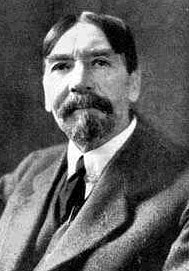
\includegraphics[width=1\textwidth]{veblen}
     \end{center}
\end{column}
\end{columns}
\end{frame}

\begin{frame}{Товары Гиффена}
\begin{columns}
\begin{column}{0.5\textwidth}
   \alert{Роберт Гиффен} (Robert Giffen) шотландский статистик и экономист конца 19 века. Среди экономистов известен \alert{парадоксом Гиффена}, заключавшичся в том, что ирландцы покупали больше картошки, когда цена картошки выросла. В отличие от Веблена, картошка - не статусный, а, наоборот, инфериорный товар. \alert{Мы вернемся к этому в 4 лекции}.

\end{column}
\begin{column}{0.5\textwidth}  %%<--- here
    \begin{center}
     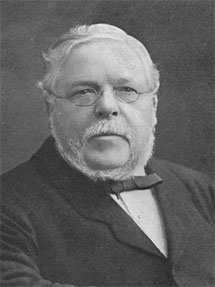
\includegraphics[width=1\textwidth]{giffen}
     \end{center}
\end{column}
\end{columns}
\end{frame}

\section{Косвенная полезность}

\begin{frame}{Косвенная полезность}

В каждой задаче оптимизации есть два объекта, идущие рука об руку: координаты оптимума и значение целевой функции (полезности). Мы довольно много внимания уделили координатам оптимума, то есть кривым спроса. 

А как насчет второго?

\begin{definition}
Назовем \alert{косвенной полезностью} значение целевой функции в оптимуме в задаче максимизации полезности:
$$ V(p,q,I) = U(x^{\ast}, y^{\ast}).$$
\end{definition}
Иногда я могу также использовать символ $U^{\ast}$.

\end{frame}

\begin{frame}{Косвенная полезность}

На самом деле, не столь важно какой буквой обозначается косвенная полезность: $U^{\ast}$ или $V$. Гораздо важнее набор аргументов: $p,q, I$, подсказывающий, что координатам $x,y$ были присвоены какие-то значения в процессе оптимизации.


Внимание! В отличие от координат оптимума, косвенная полезность, конечно же зависит от всех монотонных преобразований, которые вы наложили на свою полезность.

Если вы применили преобразование, например, $\log x$, чтобы быстрее решить задачу, и получили косвенную полезность, то вам придется ее откатить, то есть применить к ней обратное преобразование $e^x$, чтобы ответ был формально верным.

\end{frame}

\section{Непрерывность спроса}

\begin{frame}{Непрерывность спроса}

В большей часть примеров, которые мы будем рассматривать, спросы будут выражаться через элементарные функции, такие как $x^2, \log x, 1/x$... Все эти функции непрерывны. Совпадение?

Ответить на этот вопрос нам поможет \textbf{Теорема Максимума}: в \textbf{строго выпуклой} задаче оптимизации, решение, если оно существует, то единственно. Более того, если \textbf{задача непрерывна} по параметрам, то как координаты оптимума, так и значение целевой функции непрерывны по параметрам.

Я буду иногда пользоваться следующими неформальными определениями: в строго выпуклой задаче, функция $U$ (квази) вогнутa, функция $B$ (квази) выпукла, причем одна из двух строго. В непрерывной задаче обе функции $U$ и $B$ непрерывны.

\end{frame}

\section{Кривая Энгеля}

\begin{frame}{Кривая Энгеля}

Если взять две кривые доход-потребление: $x^{\ast}(I), y^{\ast}(I)$, то получится параметрически заданная кривая в пространстве товаров $(x,y)$. 

Вот эта кривая и называется кривой Энгеля.

\end{frame}

\section{Кобб-Дуглас}

\begin{frame}{Кобб-Дуглас}

\begin{definition}
Полезностью \textbf{Коббп-Дугласа} называется:
$$U(x, y) = x^{\alpha} y^{1-\alpha}, \quad \alpha \in (0,1)$$  
\end{definition}

Вспомним, что монотонные преобразования полезности не меняют поведение потребителя. Тогда можно применить логарифм и получить:
$$ U(x, y) = \alpha \log x + (1-\alpha) \log y, \quad \alpha \in (0,1).$$ 
Заметим, что эта функция вогнута!!! 
\end{frame}

\begin{frame}{Кобб-Дуглас}

Выпишем Лагранжиан:
$$ \mathcal{L} = \alpha \log x + (1-\alpha) \log y - \lambda (px + qy -I).$$ 

Заметим, что я выставляю знак минус так, чтобы у множителя Лагранжа была интерпретация теневой цены выхода за бюджетное ограничение. Это нам пригодится в следующей лекции, а сейчас просто постарайтесь запомнить.
\end{frame}

\begin{frame}{Кобб-Дуглас}

Бездумно выпишем три уравнения:

$\mathcal{L}'_x = \alpha/ x - \lambda p = 0$

$\mathcal{L}'_y = (1-\alpha)/y - \lambda q = 0$

$\mathcal{L}'_{\lambda} = I - p x - qy = 0$

Легко видеть, что они эквивалентны

$\alpha - \lambda p x= 0$

$(1-\alpha) - \lambda q y= 0$

$px + qy - I = 0$

\end{frame}

\begin{frame}{Кобб-Дуглас}

Обозначим доли бюджета потраченные на $x$ и $y$ как $s_x= px$ и $s_y = qy$ соответственно, и умножим последнее уравнение на $\lambda$. 

Тогда уравнения становятся еще проще:

$\alpha = \lambda s_x$

$(1-\alpha) = \lambda s_y$

$\lambda s_x + \lambda s_y = \lambda I$

Эту систему можно уже решить в уме. 

Получается, что теневая цена равна $\lambda = 1/I$, а доли бюджета, потраченные на каждый товар, постоянны и равны $\alpha$ и $1-\alpha$.

Это интуитивно?

\end{frame}

\begin{frame}{Кобб Дуглас}

Пусть полезность имеет следующий вид:
$$U(x,y,z) = \alpha \log x + \beta \log y + \gamma \log z$$ 
а цены равны $p, q, r$ соответственно.

Спрос на каждый товар в Коббе-Дугласе описывается следующими уравнениями:
\begin{gather*}
x^{\ast} = \frac{\alpha}{\alpha + \beta + \gamma} \frac{I}{p}, \quad
y^{\ast} = \frac{\beta}{\alpha + \beta + \gamma} \frac{I}{q}, \quad
z^{\ast} = \frac{\gamma}{\alpha + \beta + \gamma} \frac{I}{r}
\end{gather*}

Такое лучше запомнить наизусть. Также постарайтесь ответить, являются ли такие товары нормальными, комплементами или субститутами.

\end{frame}

\begin{frame}{Кобб Дуглас}

Нампомним, что косвенная полезность чувствительна к монотонным преобразованиям, поэтому тут важно какая именно спецификация была изначально дана в задаче. 

Для простоты давайте считать, что это спецификация в логарифмах.

Сосчитаем логарифм спроса на первый товар:
$$\log x^{\ast} = \log \alpha - \log (\alpha + \beta + \gamma) + \log I - \log p$$
Аналогично считается логарифм спроса на другие товары. Теперь надо просто подставить их в полезность.

\end{frame}

\begin{frame}{Кобб Дуглас}

Косвенная полезность в Коббе-Дугласе (с точностью до преобразования) имеет вид
$$V(p,q,r,I) = (\alpha + \beta + \gamma) \log I - \alpha \log p - \beta \log q - \gamma \log r + C $$
Константы $C$ можно, как правило, не выписывать, так как они исчезнут при первой же попытке продифференцировать.

Эта формула нам будет очень полезна в будущем...
\end{frame}

\section{Леонтьев}

\begin{frame}{Леонтьев}

\begin{definition}
Полезностью \textbf{Леонтьева} называется:
$$U(x, y) = \min(x/a, y/b)$$  
\end{definition}

Интерпретация полезности такая, что для извлечения одной единицы полезности необходимо ровно a и b единиц потребительских товаров. Иногда такая полезность называется \textbf{совершенными комплементами}.

\end{frame}

\begin{frame}{Леонтьев}

\begin{figure}[hbt]
\centering
\includegraphics[width=.8 \textwidth]{leontiev}
\end{figure}

\end{frame}

\begin{frame}{Леонтьев}

Поскольку задача негладкая, то геометрический метод проще и быстрее. Решение лежит в пересечении кривой Энгеля и бюджетной линии. 

Соответственно, достаточно решить систему уравнений:
$$ px + qy = I, \quad b x = a y$$
Кривая Энгеля здесь – это множество точек, от которых отложены уголки.

\end{frame}

\begin{frame}{Леонтьев}

Пусть полезность имеет следующий вид:
$$U(x,y,z) = \min(x/a, y/b, z/c)$$ 
а цены равны $p, q, r$ соответственно. 

Спрос на каждый товар в Леонтьеве описывается следующими уравнениями:
\begin{gather*}
x^{\ast} = \frac{ap}{ap + bq + cr} \frac{I}{p}, \\
y^{\ast} = \frac{bq}{ap + bq + cr} \frac{I}{q}, \\
z^{\ast} = \frac{cr}{ap + bq + cr} \frac{I}{r}.
\end{gather*}

Все товары в функции Леонтьева являются нормальными, а также попарно являются (строго) комплементами.

\end{frame}

\begin{frame}{Леонтьев}

Заметим, что в оптимуме полезности в обоих позициях аргумента одинаковые. То есть косвенная полезность равна одновременно левому и правому аргументу.


Косвенная полезность в Леонтьеве (с точностью до преобразования) имеет вид
$$V(p,q,I) = \frac{I}{ap + bq + cr}$$

Это тоже очень полезная формула.

\end{frame}

\section{Квазилинейная}

\begin{frame}{Квазилинейная}

Пожалуй, третья самая важная полезность имеет следующий вид:

\begin{definition}
\textbf{Квазилинейной полезностью} называется:
$$U(x, y) = f(x) + k y,$$ 
где $f$ - вогнутая функция.
\end{definition}

Интерпретация последней координаты - это деньги на счету. То есть вам не обязательно тратить весь бюджет как раньше и остаток средств на счету конвертируется в утили по курсу 1:$k$.

\end{frame}

\begin{frame}{Квазилинейная}

Выпишем Лагранжиан:
$$\mathcal{L} = f(x) + k y - \lambda (px + y - I).$$ 
Легко, правда?

Обратите внимание, что цена денег равна единице.

\end{frame}

\begin{frame}{Квазилинейная}

Сейчас мы попробуем найти внутреннее решение.

$\mathcal{L}'_x = f'_x - \lambda p = 0$

$\mathcal{L}'_y = k - \lambda = 0$

$\mathcal{L}'_{\lambda} = I - p x - y= 0$

Легко видеть, что они эквивалентны

$k = \lambda$

$x = (f')^{-1}(\lambda p)$

$px + y = I$

\end{frame}

\begin{frame}{Квазилинейная}

Сейчас мы попробуем найти внутреннее решение.

$\mathcal{L}'_x = f'_x - \lambda p = 0$

$\mathcal{L}'_y = k - \lambda = 0$

$\mathcal{L}'_{\lambda} = I - p x - y= 0$

Легко видеть, что они эквивалентны

$k = \lambda$

$x = (f')^{-1}(\lambda p)$

$px + y = I$

\end{frame}

\begin{frame}{Квазилинейная}

Однако эта система не всегда имеет решение в $\mathbb{R}^2_{+}$. Легко видеть, что спрос на товар $x$ никак не зависит от бюджета, а стало быть, при достаточно маленьком бюджете спрос на товар $y$ упрется в ноль.

Мы оказались в ситуации, о которой я предупреждал. Условия первого порядка указали на точку, которая может оказаться вне допустимой области. Если это так, это значит что решение не внутреннее, а краевое. В таком случае, мы заменяем условие первого порядка  $x = (f')^{-1}(\lambda p)$ на краевое условие $y=0$ или эквивалентно $x = I/p$.

\end{frame}


\begin{frame}{Квазилинейная}

В этой задаче есть два взаимоисключающих режима: внутреннее решение и краевое решение. Но вместо перебора случаев, можно записать ответ в компактной форме, если проявить немного смекалки.

Спрос на каждый товар в квазилинейной полезности описывается следующими уравнениями:
\begin{gather*}
x^{\ast} = \min (I/p, (f')^{-1}(k p)), \\
y^{\ast} = \max (0, I-px^{\ast}).
\end{gather*}
Все товары в квазилинейной полезности являются нормальными, a деньги (переменная $y$) являются универсальным комплементом.
\end{frame}

\begin{frame}{Квазилинейная}

Поскольку в задаче два режима, скорее всего ответ будет иметь форму максимума или минимума из двух выражений. Если бы ограничения не было, решение было бы всегда внутреннее, а полезность равна 
$$f((f')^{-1}(k p)) + I - p (f')^{-1}(k p).$$

Когда ограничение активно, оно мешает нам достигнуть этой полезности и мы получаем вместо нее
$$ f(I/p) + 0.$$

\end{frame}

\section{Линейная}

\begin{frame}{Линейная}

Простая с виду, но очень неудобная на практике:

\begin{definition}
\textbf{Линейной полезностью} называется:
$$U(x, y) = x/a +y/b,$$ 
\end{definition}

интерпретируется как способность извлекать одну и туже полезность из разных источников.  Конкретно вы можете получить одну единицу полезности либо из $a$ единиц товара $x$, либо из $b$ единиц товара $y$. 

Это значит, что $x, y$ обладают высокой взаимозаменяемостью либо вообще представляют собой один и тот же товар в пачках/таре разного размера. Такая полезность еще часто называется \textbf{совершенными субститутами}.

\end{frame}

\begin{frame}{Линейная}

Решение в этой задаче не похоже на предыдущие, оно вообще всегда краевое. 

Почему так? Посмотрим внимательно на бюджетное ограничение:

$$B(x,y) = px + qy - I \leqslant 0$$ 

оно показывает, что вы можете менять товары $x, y$ по курсу $\frac{1}{p}$ к $\frac{1}{q}$. А в полезности вы можете менять товары по курсу $a$:$b$. За исключением редкого случая, когда эти курсы совпадают: 
$$ap = bq,$$ 
вам выгодно менять один товар на другой до упора.
\end{frame}

\begin{frame}{Линейная}

Осталось понять, каким будет краевое решение...

Интуитивно понятно, что вы будете тратить все на $x$, когда его вес в полезности относительно большой, а его цена относительно маленькая. То есть, когда $ap$ относительно маленький. 

Относительно чего? Конечно же, относительно $bq$.

\end{frame}

\begin{frame}{Линейная}

Осталось понять, каким будет краевое решение...

Интуитивно понятно, что вы будете тратить все на $x$, когда его вес в полезности относительно большой, а его цена относительно маленькая. То есть, когда $ap$ относительно маленький. 

Относительно чего? Конечно же, относительно $bq$.

Спрос на каждый товар описывается так: 

если $ap < bq$, то $x^{\ast} = I/p, y^{\ast} = 0$

если $ap > bq$, то $x^{\ast} = 0, y^{\ast} = I/q$

Все товары в линейной полезности нормальные и являются попарно субститутами.

\end{frame}

\begin{frame}{Линейная}

Мы знаем, что решение либо в одном углу, либо в другом. Соответственно, ответ это наибольшая из двух полезностей этих кандидатов, то есть
$$V(p,q,I) = I \cdot \max(\frac{1}{ap}, \frac{1}{bq}).$$
Пользуясь тем, что максимум коммутирует с монотонно возрастающими преобразованиями
$$ \varphi'(x) >0 \quad \Rightarrow \quad \max(\varphi(x), \varphi(x)) = \varphi(\max(x, y)$$
и с монотонно убывающими преобразованиями в некотором смысле тоже
$$ \psi'(x) < 0 \quad \Rightarrow \quad \max(\psi(x), \psi(x)) = \psi(\min(x, y)$$
можно вывести следующее красивое свойство...

\end{frame}

\begin{frame}{Линейная}

Косвенная полезность в линейной полезности (с точностью до преобразования) имеет вид
$$V(p,q,I) = I / \min(ap, bq),$$
Это тоже лучше запомнить наизусть.
\end{frame}

\section{Конец}

\end{document}